\documentclass[11pt, oneside]{article} 
\usepackage{geometry}
\geometry{letterpaper} 
\usepackage{graphicx}
	
\usepackage{amssymb}
\usepackage{amsmath}
\usepackage{parskip}
\usepackage{color}
\usepackage{hyperref}

\graphicspath{{/Users/telliott_admin/Dropbox/Tex/png/}}
% \begin{center} 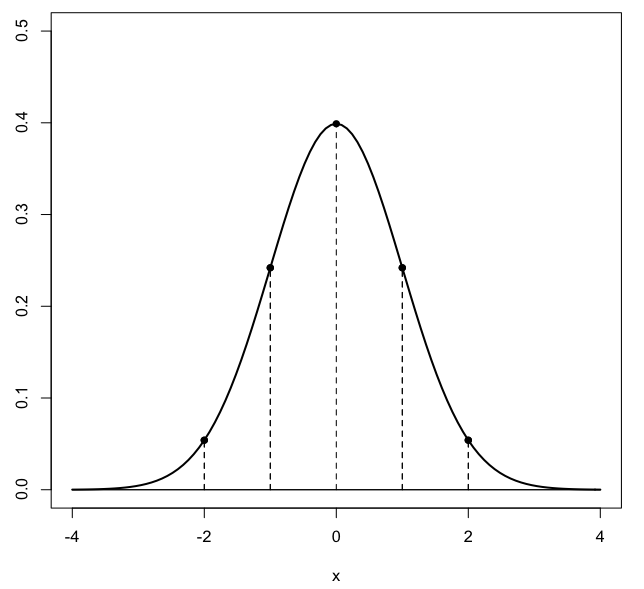
\includegraphics [scale=0.4] {gauss3.png} \end{center}

\title{Basic geometry and congruence of triangles}
\date{}

\begin{document}
\maketitle
\Large

\subsection*{Euclid and the postulates}
Greek geometry starts hundreds of years before Euclid, who was born in 323 BC, the year that Alexander the Great died. But Euclid's book \emph{Elements} is still an excellent place to begin surveying the foundations of geometry.

Euclid's geometry is mainly constructions (geometric figures) drawn with a pencil on a flat piece of paper, using a straight-edge or a compass or both.  

\begin{center} 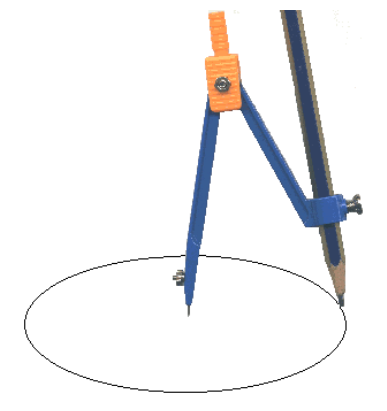
\includegraphics [scale=0.3] {compass.png} \end{center}

Here are Euclid's first three postulates --- statements that are assumed to be true:

$\circ$  A straight line segment can be drawn joining any two points.

$\circ$   Any straight line segment can be extended indefinitely in a straight line.

$\circ$   Given any straight line segment, a circle can be drawn having the segment as radius and one endpoint as center.

Let us assume these as well.

We finesse the difficulty in defining what is meant by \emph{straight} in the real world.  If you've ever done any carpentry, for example, you probably know that unknown edges are determined to be straight by comparison with known straight edges.  But the mental construct of  "a straight line is the shortest distance between two points" gets around this limitation.

The fourth postulate is:

$\circ$   All right angles are congruent, that is, equal to each other.

This one prompts a different question:  what is a "right angle"?  

If a line segment is drawn with one end on a line, let us refer to the two angles the line segment forms with the line as adjacent angles.

The definition of a right angle is this:  if these two adjacent angles are equal, then they are both right angles.

\begin{center} 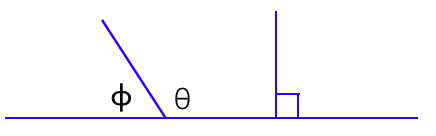
\includegraphics [scale=0.4] {perps.png} \end{center}

On the left, one of the angles, $\phi$, is smaller than the other one, $\theta$.  

Alternatively, on the right, the two angles have equal measures.  In this case we can conclude that both angles are right angles.   A right angle is frequently designated by drawing a small square at the intersection. Since both angles are right angles, only one square is needed or usually drawn.

In all cases, the sum of the two angles $\phi + \theta$ is equal to two right angles or 180 degrees.  There is nothing particularly special about $180$ degrees for two right angles or $360$ degrees for one whole turn.  

Well, there is one thing:  there are \emph{approximately} 360 days in a year, which marks the sun's track across the sky.  In his book, \emph{Measurement}, Lockhart adopts the convention that one whole turn is equal to $1$.  

Later, we'll see that one whole turn is defined as $2 \pi$ radians, and that convention turns out to be quite important.

Now, extend those lines below the horizontal

\begin{center} 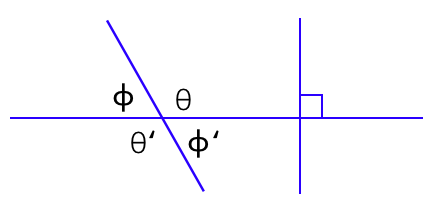
\includegraphics [scale=0.4] {perps2.png} \end{center}

We said that the sum of the two angles $\phi + \theta$ is equal to two right angles, but so is the sum $\theta + \phi'$, for the same reason.

\[ \phi + \theta = \theta + \phi' \]
We conclude that $\phi = \phi'$ and $\theta = \theta'$.  On the right, if any one of the angles where two lines cross is a right angle, then all four are right angles.

This is called the vertical angle theorem.

There is a simple method to construct a line segment perpendicular to a line at a particular (given) point, or alternatively, through any point not on the line (see the video at the url):

\url{https://www.mathopenref.com/constperpextpoint.html}

\subsection*{parallel postulate}

All this seems rather obvious.  

The fifth and final postulate is more subtle:

$\circ$   If two lines are drawn which intersect a third in such a way that the sum of the inner angles on one side is less than two right angles, then the two lines inevitably must intersect each other on that side if extended far enough.
\begin{center} 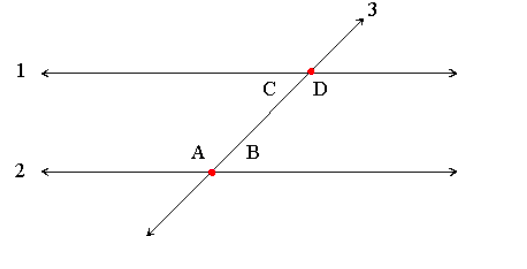
\includegraphics [scale=0.5] {alternate_interior_angles.png} \end{center}

Line $1$ and line $2$ are parallel, if and only if, $A + C = B + D = 180 = 2$ right angles.  This postulate is equivalent to what is known as the parallel postulate.

\url{http://mathworld.wolfram.com/EuclidsPostulates.html}

Consider a familiar situation where this is not true.  Suppose we are doing geometry on the surface of a sphere, such as the earth.  Two adjacent lines of longitude can be drawn so as to cross the equator at right angles, and the lines are parallel there, but they meet (intersect) at the poles.  

The parallel postulate only holds for geometry on a \emph{flat} surface.

\subsection*{axioms}

Euclid also lists five axioms.  Here are two examples:

$\circ$   Things that are equal to the same thing are also equal to one another.

$\circ$   If equals are added to equals, then the wholes are equal.

We will see how to proceed from the postulates and axioms to various proofs.  \emph{Given these assumptions}, we can prove theorems that must be true.

\subsection*{Thales}
I'm a big fan of William Dunham's books --- three of them are listed in the References.  

Dunham has written a lot about the history of mathematics in Greece, starting with Thales (624-546 BC), who was from a Greek town called Miletus on the coast of Asia Minor (modern Turkey).  He lived long before Euclid.  Although none of his writing survives, it is believed that Thales proved several early theorems including one we saw above

$\circ$  The vertical angles formed by two straight lines crossing, are equal.
\begin{center} 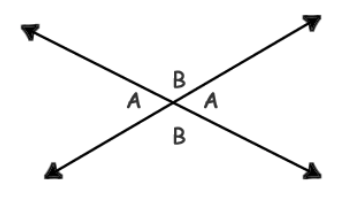
\includegraphics [scale=0.4] {vertical_angles.png} \end{center}
This theorem depends on a property of straight lines.  In the proof, we used the axiom  "equals added to equals are equal", alternatively "equals subtracted from equals are equal."

$\circ$  The angle sum of a triangle is equal to two right angles.
\begin{center} 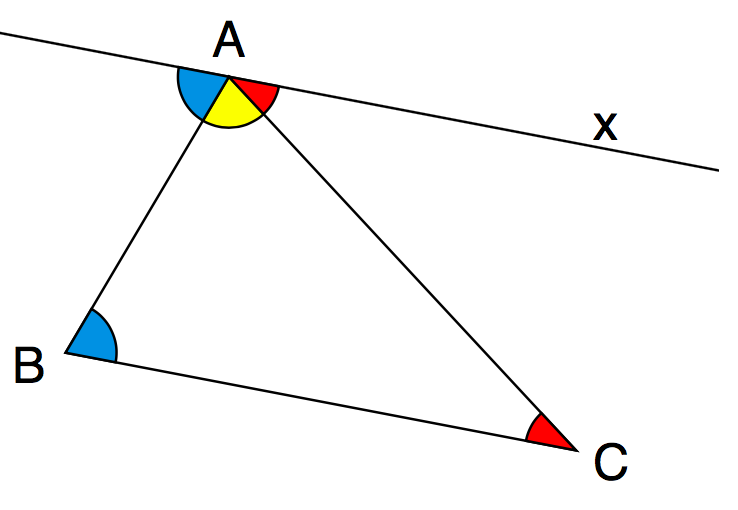
\includegraphics [scale=0.3] {triangle_sum_angles.png} \end{center}

This theorem depends in turn on a theorem which we laid the groundwork for above but did not state explicitly.

In the figure below, if $1$ is parallel to $2$, we said that $A + C = B + D = 180$ degrees.  \begin{center} 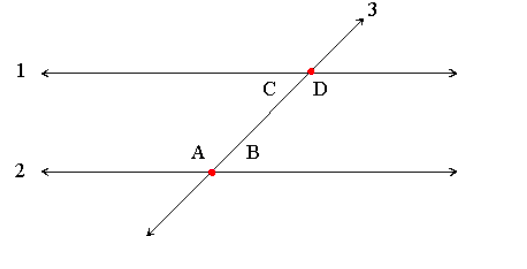
\includegraphics [scale=0.5] {alternate_interior_angles.png} \end{center}

But we also know from the properties of two lines given above that $A + B = 180$ degrees. So
\[ A + C = 180 = A + B \]
and then
\[ C = B \]

This is called the theorem on alternate interior angles.  Given this, you can go back to the angles of a triangle problem and follow the colors to the proof.

\subsection*{another proof}
Here is an alternative proof of the theorem on the sum of angles in a triangle adding to 180 degrees..

Imagine walking around the perimeter of a triangle in the counter-clockwise direction.  At each vertex we turn left by a certain number of degrees, $t$, called the exterior angle.  After passing through all three vertices, we must end up facing in the same direction as we started.

\begin{center} 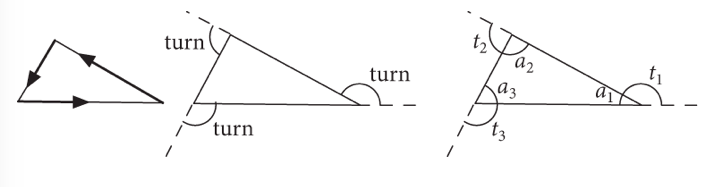
\includegraphics [scale=0.5] {triangle_sum_angles2.png} \end{center}

\[ t_1 + t_2 + t_3 = 360 \]

In addition, for each vertex, the interior angle $a_i$ plus the exterior angle $t_i$ add up to $180$ degrees.  If we add up all three pairs, we obtain
\[ (t_1 + a_1) + (t_2 + a_2) + (t_3 + a_3) = 3 \cdot 180 = 540 \]
By subtraction
\[ a_1 + a_2 + a_3 = 180 \]

\subsection*{Congruence and similarity of triangles}

$\circ$  Two triangles are \emph{congruent} if and only if they have the same three side lengths.  This is often abbreviated SSS (side-side-side).  

By this definition, a triangle and its mirror image are congruent.  The three triangles shown below are all congruent, even though the first is flipped (it is the mirror image of the other two).

\begin{center} 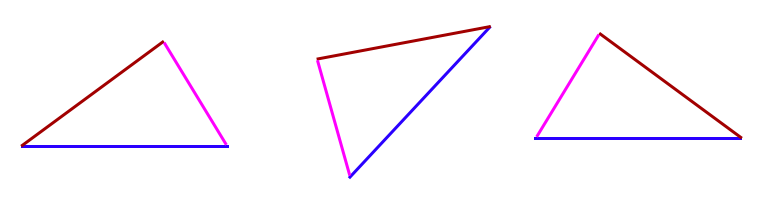
\includegraphics [scale=0.4] {congruent.png} \end{center}

Having the same three sides means that the shape is the same, and all three angles are the same --- the shapes are superimposable, with the proviso that we allow the shape to be flipped over.

Some triangles are \emph{similar} but not congruent, with all three angles the same but of different overall sizes.  We could call this AAA (angle-angle-angle).  For similar triangles, the three corresponding pairs of sides are in the same proportions, but scaled differently.

$\circ$  Two triangles are similar if they have the same three angles. 

Because of the angle sum theorem, if any two angles of a pair of triangles are known to be equal, then the third one must be equal as well.

Similar triangles have their sides in the same proportions.

\begin{center} 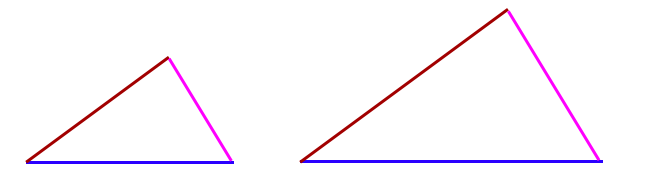
\includegraphics [scale=0.4] {similar.png} \end{center}

Given any triangle, draw a line parallel to one side, which also joins the other two sides.  The new triangle is similar to the given triangle.  Similarity means that all the angles are equal.  This is easily proved using the theorem on alternate interior angles.

\begin{center} 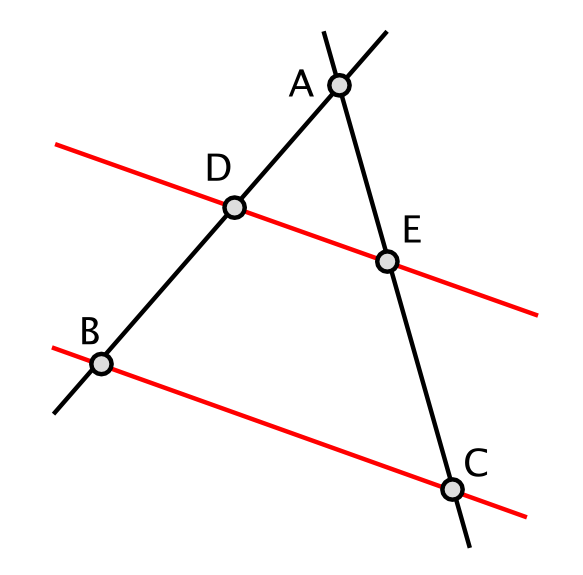
\includegraphics [scale=0.25] {Thales_theorem_1.png} \end{center}
%\begin{center} 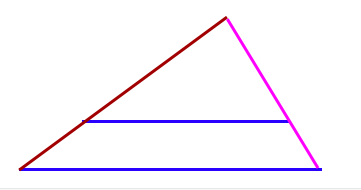
\includegraphics [scale=0.4] {parallel_line.png} \end{center}

In this example, these ratios are all equal
\[ \frac{AD}{DB} = \frac{AE}{EC} = \frac{DE}{BC} =  \]

In addition to SSS (side-side-side), there are other conditions that lead to congruence of two triangles when they are satisfied, namely

$\circ$  SAS (side-angle-side)

$\circ$  ASA (angle-side-angle)

$\circ$  AAS (angle-angle-side)

\subsection*{constructions}

Again, the way I think about these conditions is to imagine trying to construct a triangle from the given information, and ask whether it is uniquely determined.  Suppose we know ASA.  The situation is thus:

\begin{center} 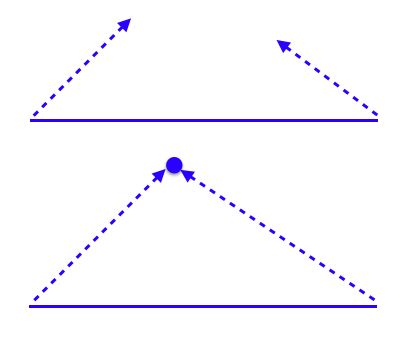
\includegraphics [scale=0.4] {ASA.png} \end{center}
 
Plot the known side and start two other sides from the ends of that side containing the known angles.  They must cross at a unique point.  

But... actually, if we start the two lines pointing below the horizontal, there is another solution, the mirror image.  This triangle is also congruent to the one above.
 
\begin{center} 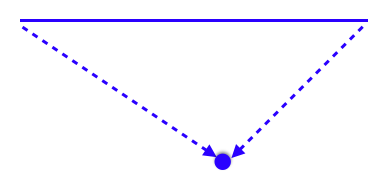
\includegraphics [scale=0.4] {ASA2.png} \end{center}

Alternatively, knowing two angles means we also know the third, because they must add to 180 degrees.  For this reason, ASA and AAS imply that we have exactly the same information, because we know all three angles and (this part is important) we also know \emph{which} two angles flank the known side.
 
For a right-triangle, if the hypotenuse and one leg are equal, the two triangles are congruent.

\begin{center} 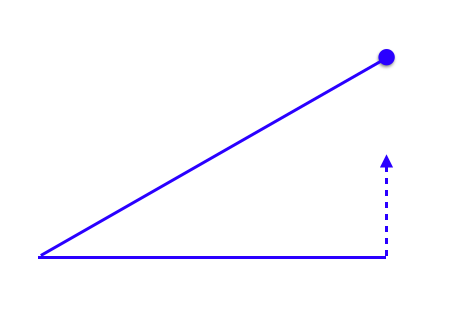
\includegraphics [scale=0.4] {hyp_side_congruent.png} \end{center}

In the figure, imagine the hypotenuse swinging on the hinge of its vertex with the horizontal base.  There is only one angle where it will terminate on the vertical side with the correct length.  This determines the angle between the known sides, or alternatively, the length of the third side.
 
\subsection*{another theorem from Thales}

$\circ$  The base angles of an isosceles triangle are equal.

\begin{center} 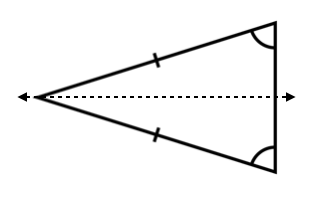
\includegraphics [scale=0.6] {isosceles.png} \end{center}
My favorite proof of this theorem is from symmetry.  Draw a line from the vertex between the two equal sides to the midpoint of the base opposite.  If you turn the triangle over along this axis, we obtain the same triangle back again.  Alternatively, just say "side-side-side."

Euclid's proof is here:

\begin{center} 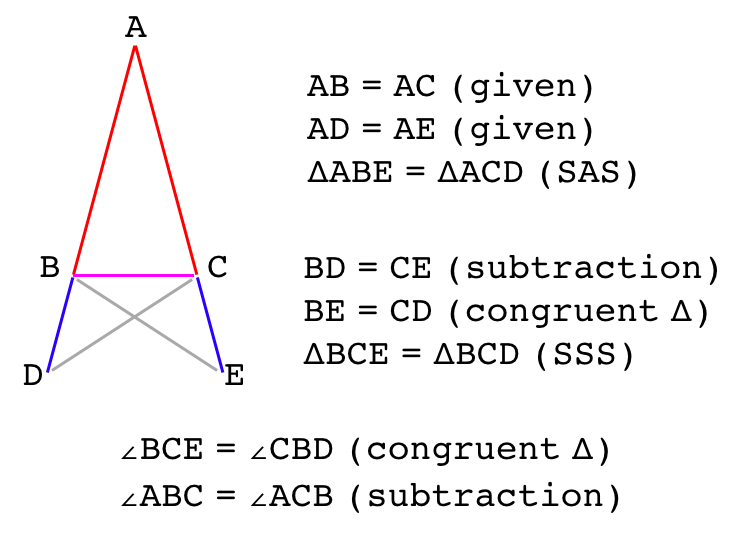
\includegraphics [scale=0.4] {isosceles_proof.png} \end{center}

\subsection*{pyramid height}
As we said, Thales was from Miletus and he lived around 600 BC.  Thales is believed to have traveled extensively around the Mediterranean and was probably of Phoenician heritage, famous sailors.  

During his travels, he went to Egypt, home to the great pyramids at Giza, which were already ancient then.  They were built just around around 2560 BC (dated by reference to Egyptian kings) and were already 2000 years old at that time!

The story is that Thales asked the Egyptian priests about the height of the Great Pyramid of Cheops, and they would not tell him.  So he set about measuring it himself.  The current height is 480 feet.  He used similar triangles.

\begin{center} 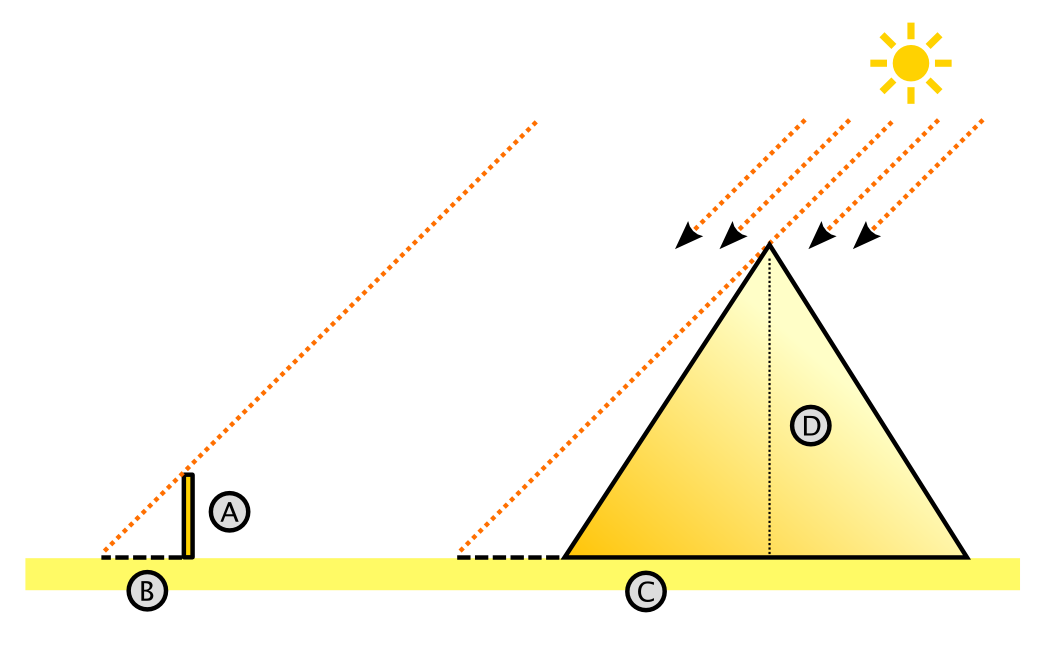
\includegraphics [scale=0.25] {Thales_theorem_6.png} \end{center}

\subsection*{platonic solids}

\url{https://en.wikipedia.org/wiki/Platonic_solid}

\begin{quote}
In three-dimensional space, a Platonic solid is a regular, convex polyhedron. It is constructed by congruent (identical in shape and size) regular (all angles equal and all sides equal) polygonal faces with the same number of faces meeting at each vertex. Five solids meet these criteria.
\end{quote}

\begin{center} 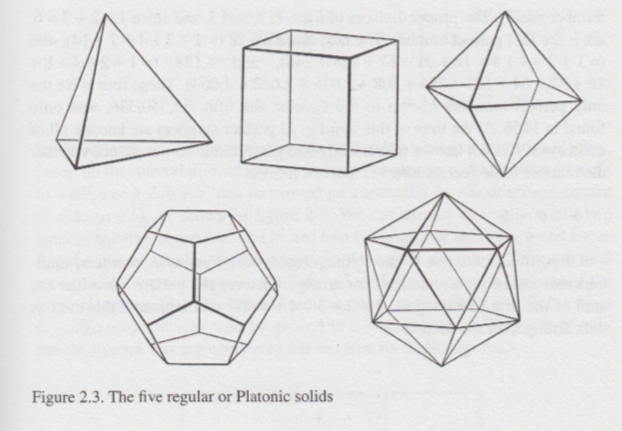
\includegraphics [scale=0.5] {platonic_solids.png} \end{center}
These are:  (i) tetrahedron, (ii) cube, (iii) octagon, (iv) dodecagon, and (v) icosahedron.

There is a wonderful, simple proof that there are only five of them.  Any solid requires at least three sides meeting at each vertex, otherwise the joint between two sides can just flap, like a hinge.  Furthermore, the total of all the vertex angles added up must be less than $360$ degrees.

So, three equilateral triangles total $60 \times 3 = 180$, four total $60 \times 4 = 240$ and five total $60 \times 5 = 300$.  Six would be a hexagon lying in the plane.  Three squares total $90 \times 3 = 270$, while four give a square array in the plane.  Finally, three pentagons give $108 \times 3 = 324$.  And that's it.  Three hexagons would give $120 \times 3 = 360$, which gives an array in the plane.

Proving that all the angles and side lengths come out correctly, so that the possible solids actually can be constructed is another matter, however.  Euclid devotes book XIII of \emph{The Elements} to this:

\url{https://mathcs.clarku.edu/~djoyce/elements/bookXIII/bookXIII.html#props}


\end{document}